\documentclass[12pt]{beamer}
\usepackage[utf8]{inputenc}
\usepackage[spanish]{babel}
\usepackage{amsmath}
\usepackage{amsfonts}
\usepackage{amssymb}
\usepackage{graphicx}
\usepackage{mathrsfs} 
\usepackage{outlines}
\usetheme{Goettingen}
\DeclareMathOperator{\re}{Re}
\begin{document}
	\author{Carlos Daniel Contreras Quiroz}
	\title{Desarrollo de un programa de lectura y análisis de películas radiocrómicas para verificación dosimétrica}
	%\subtitle{}
	\logo{
\includegraphics{images/logo.png}}
	\institute{Universidad de los Andes}
	%\date{}
	%\subject{}
	%\setbeamercovered{transparent}
	%\setbeamertemplate{navigation symbols}{}
	\begin{frame}[plain]
	\maketitle
\end{frame}

\begin{frame}{Contenido}
\tableofcontents
\end{frame}

\section{Introducción}
\begin{frame}
\vfill
\centering
\begin{beamercolorbox}[sep=8pt,center,shadow=true,rounded=true]{title}
	\usebeamerfont{title}\insertsectionhead\par%
\end{beamercolorbox}
\vfill
\end{frame}
\subsection{Objetivos}

\begin{frame}{Motivación}
Los planes de tratamiento con radioterapia requieren de una alta precisión en las dosis entregadas, desviaciones menores al $5\%$.  \\~\\

Es conveniente implementar sistemas que permitan verificar que los planes de tratamiento se cumplan con suficiente veracidad.

\end{frame}

\begin{frame}{Motivación}
	Existen diversos mecanismos para realizar el monitoreo de geometrías y dosis entregadas.\\
	\begin{itemize}
		\item Detectores de silicio
		\item Detectores con cámaras de ionización 
	\end{itemize}
	Sin embargo, a veces son muy costosos o no proporcionan la resolución suficiente para ciertas aplicaciones.
\end{frame}

\begin{frame}{Motivación}
	Una posible solución es el uso de películas radiocrómicas 
	\begin{figure}
		\centering
		
\includegraphics[width=0.7\linewidth]{images/fondoblancoLandscape-1.png}
	\end{figure}
\end{frame}

\begin{frame}{Motivación}
	\begin{figure}
		\centering
		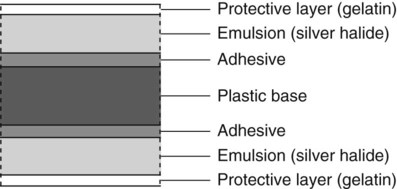
\includegraphics[width=0.7\linewidth]{images/radiographic-film.jpg}
	\end{figure}
\end{frame}

\begin{frame}{Motivación}
\begin{figure}
	\centering
	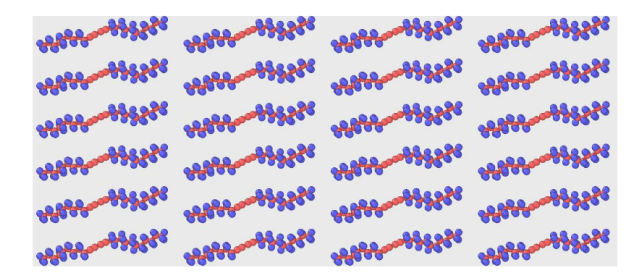
\includegraphics[width=\linewidth]{images/diacetileno.png}
\end{figure}
\end{frame}

\begin{frame}{Motivación}
	El uso de estas presenta varias ventajas
	\begin{itemize}
		\item Alta sensibilidad a la dosis y resolución espacial
		\item Bajo costo (relativamente)
		\item Practicas de usar
	\end{itemize}
\end{frame}

\begin{frame}{Objetivos}
	\begin{outline}
		\1 Entender y aplicar el funcionamiento de películas radiocrómicas en verificación dosimétrica
		\2 Realizar calibraciones de dosis
		\2 Obtener mapas de dosis de un tratamiento a partir de una película
		\2 Realizar la comparación con el plan esperado
		\1 Desarrollar un software que permita su uso bajo diferentes modalidades para su uso en el CCC
	\end{outline}
\end{frame}


\subsection{Tratamiento de películas radiocrómicas}
\begin{frame}{Modo de uso de películas radiocrómicas}
Para usar la películas hay que tener en cuenta ciertos factores ambientales que afectan las medidas
	\begin{outline}
		\1 Temperatura
		\1 Humedad
		\1 Orientación de escaneo
		\1 \textbf{Tiempo post-irradiación}
	\end{outline}
Mantenerlos controlados basta para una medida precisa
\end{frame}

\begin{frame}{Calibración}
	Irradiamos la película con diferentes dosis conocidas, obtenemos cierta coloración por cada dosis
	\begin{figure}
		\centering
		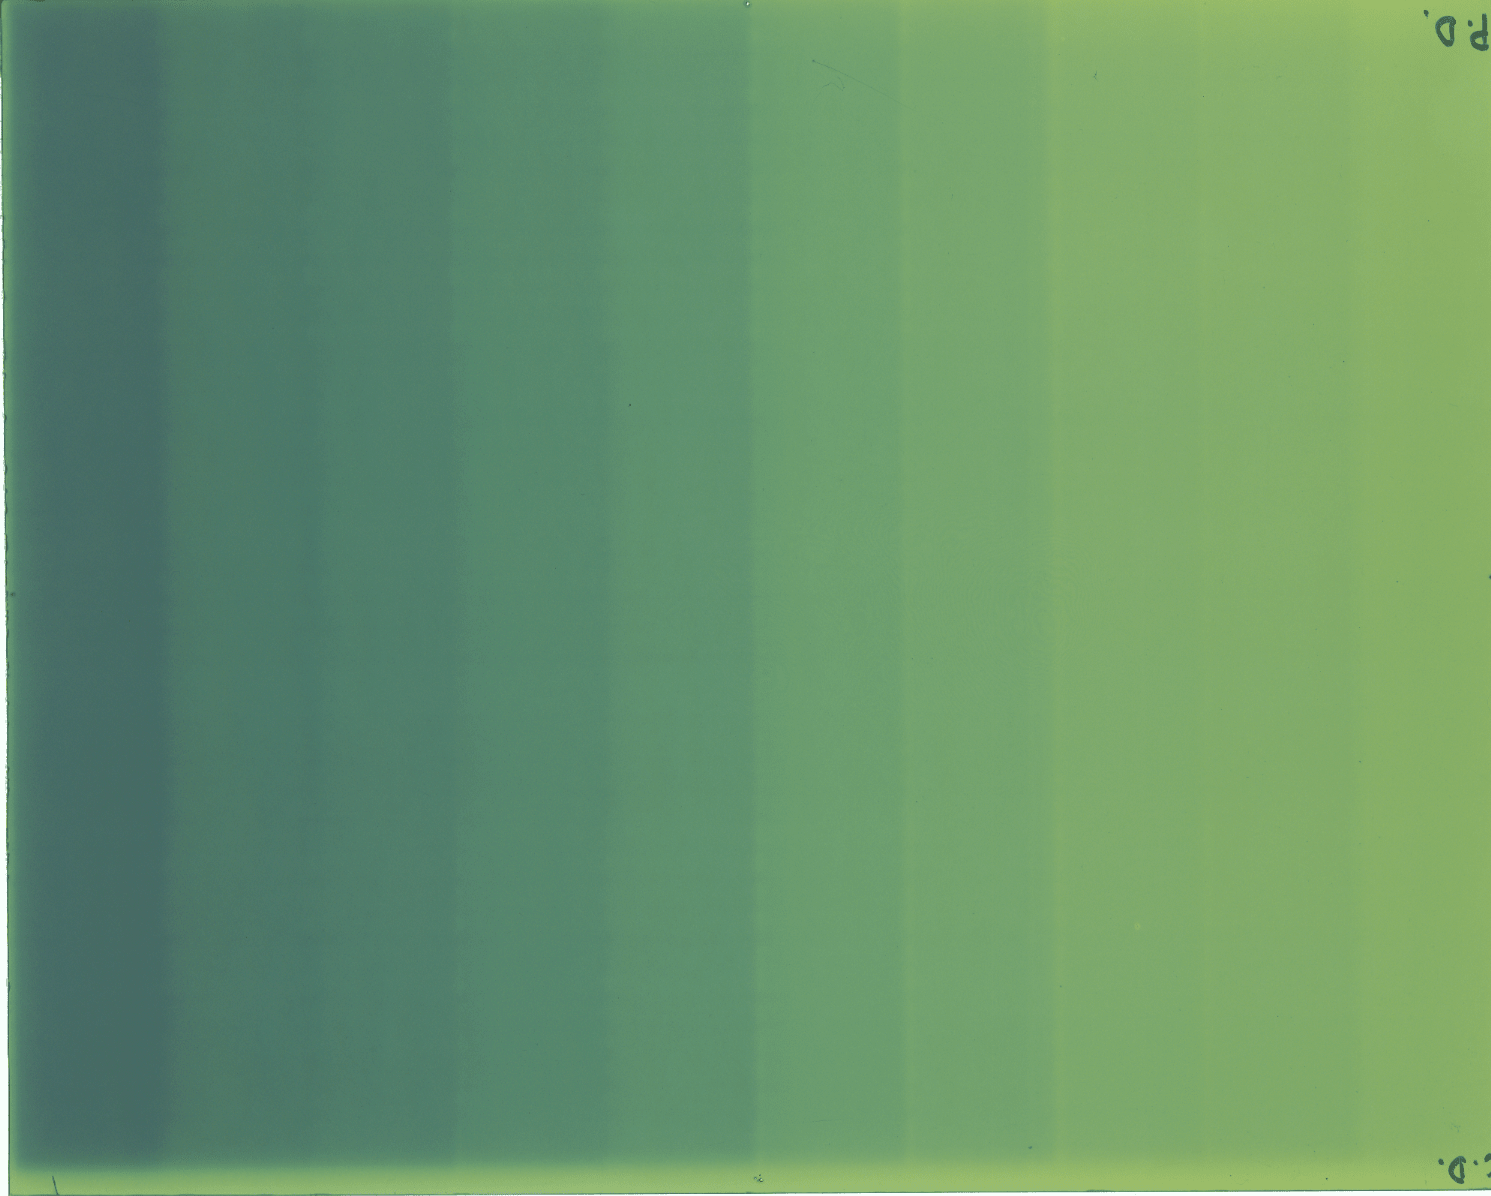
\includegraphics[width=\linewidth]{images/calibracionSimpleLandscape.png}
	\end{figure}
\end{frame}

\begin{frame}{Método general}
	Promediamos los colores en los tres canales y los asociamos a cada dosis
	\begin{figure}
		\centering
		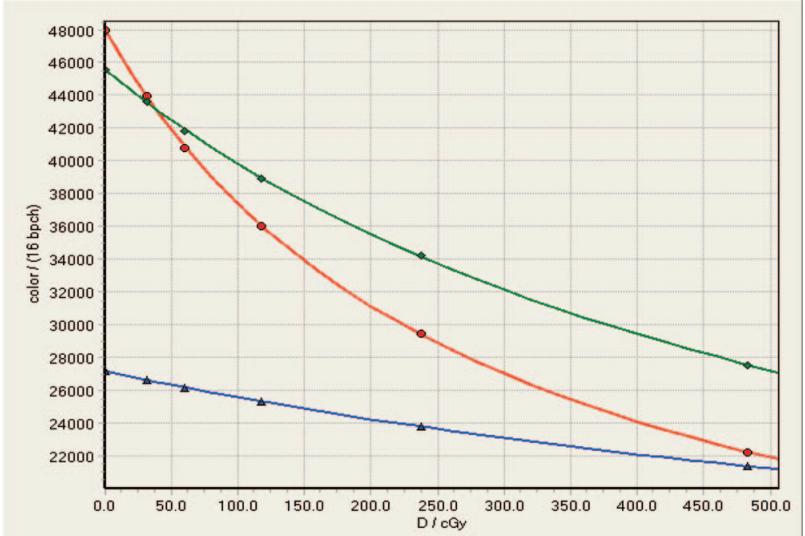
\includegraphics[width=\linewidth]{images/respses.png}
	\end{figure}
\end{frame}

\begin{frame}
	Se correlacionan los datos mediante un ajuste a algún tipo de curva.\\
	Estos son los tipo de funciones más usadas
	\begin{itemize}
		\item Racionales 
		\item Polinomicas
		\item Inversas
		\item Lineal
	\end{itemize}
\end{frame}

\begin{frame}
	Con esta curva podemos relacionar dosis con colores en una película irradiada.\\~\\
	Con esta podemos generar mapas de dosis
	\begin{figure}
		\centering
		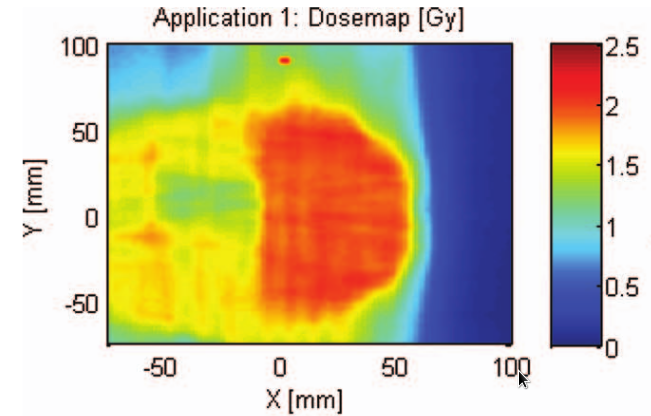
\includegraphics[width=0.7\linewidth]{images/dosemap.png}
	\end{figure}
\end{frame}


\begin{frame}{Métodos Corregidos}
Podemos sofisticar un poco con correcciones como 
\begin{itemize}
	\item Usar información de los tres canales para corregir inhomogeneidades
	\item Aplicar cambios en las curvas para incluir errores laterales en el escáner
	\item Filtrar las imágenes para corregir defectos
\end{itemize}
\end{frame}

\section{Avances}
\begin{frame}
	\vfill
	\centering
	\begin{beamercolorbox}[sep=8pt,center,shadow=true,rounded=true]{title}
		\usebeamerfont{title}\insertsectionhead\par%
	\end{beamercolorbox}
	\vfill
\end{frame}

\subsection{Toma de imágenes}

\begin{frame}{Toma de imágenes}
Hemos tomado imágenes de prueba para la programación
\begin{figure}
	\centering
	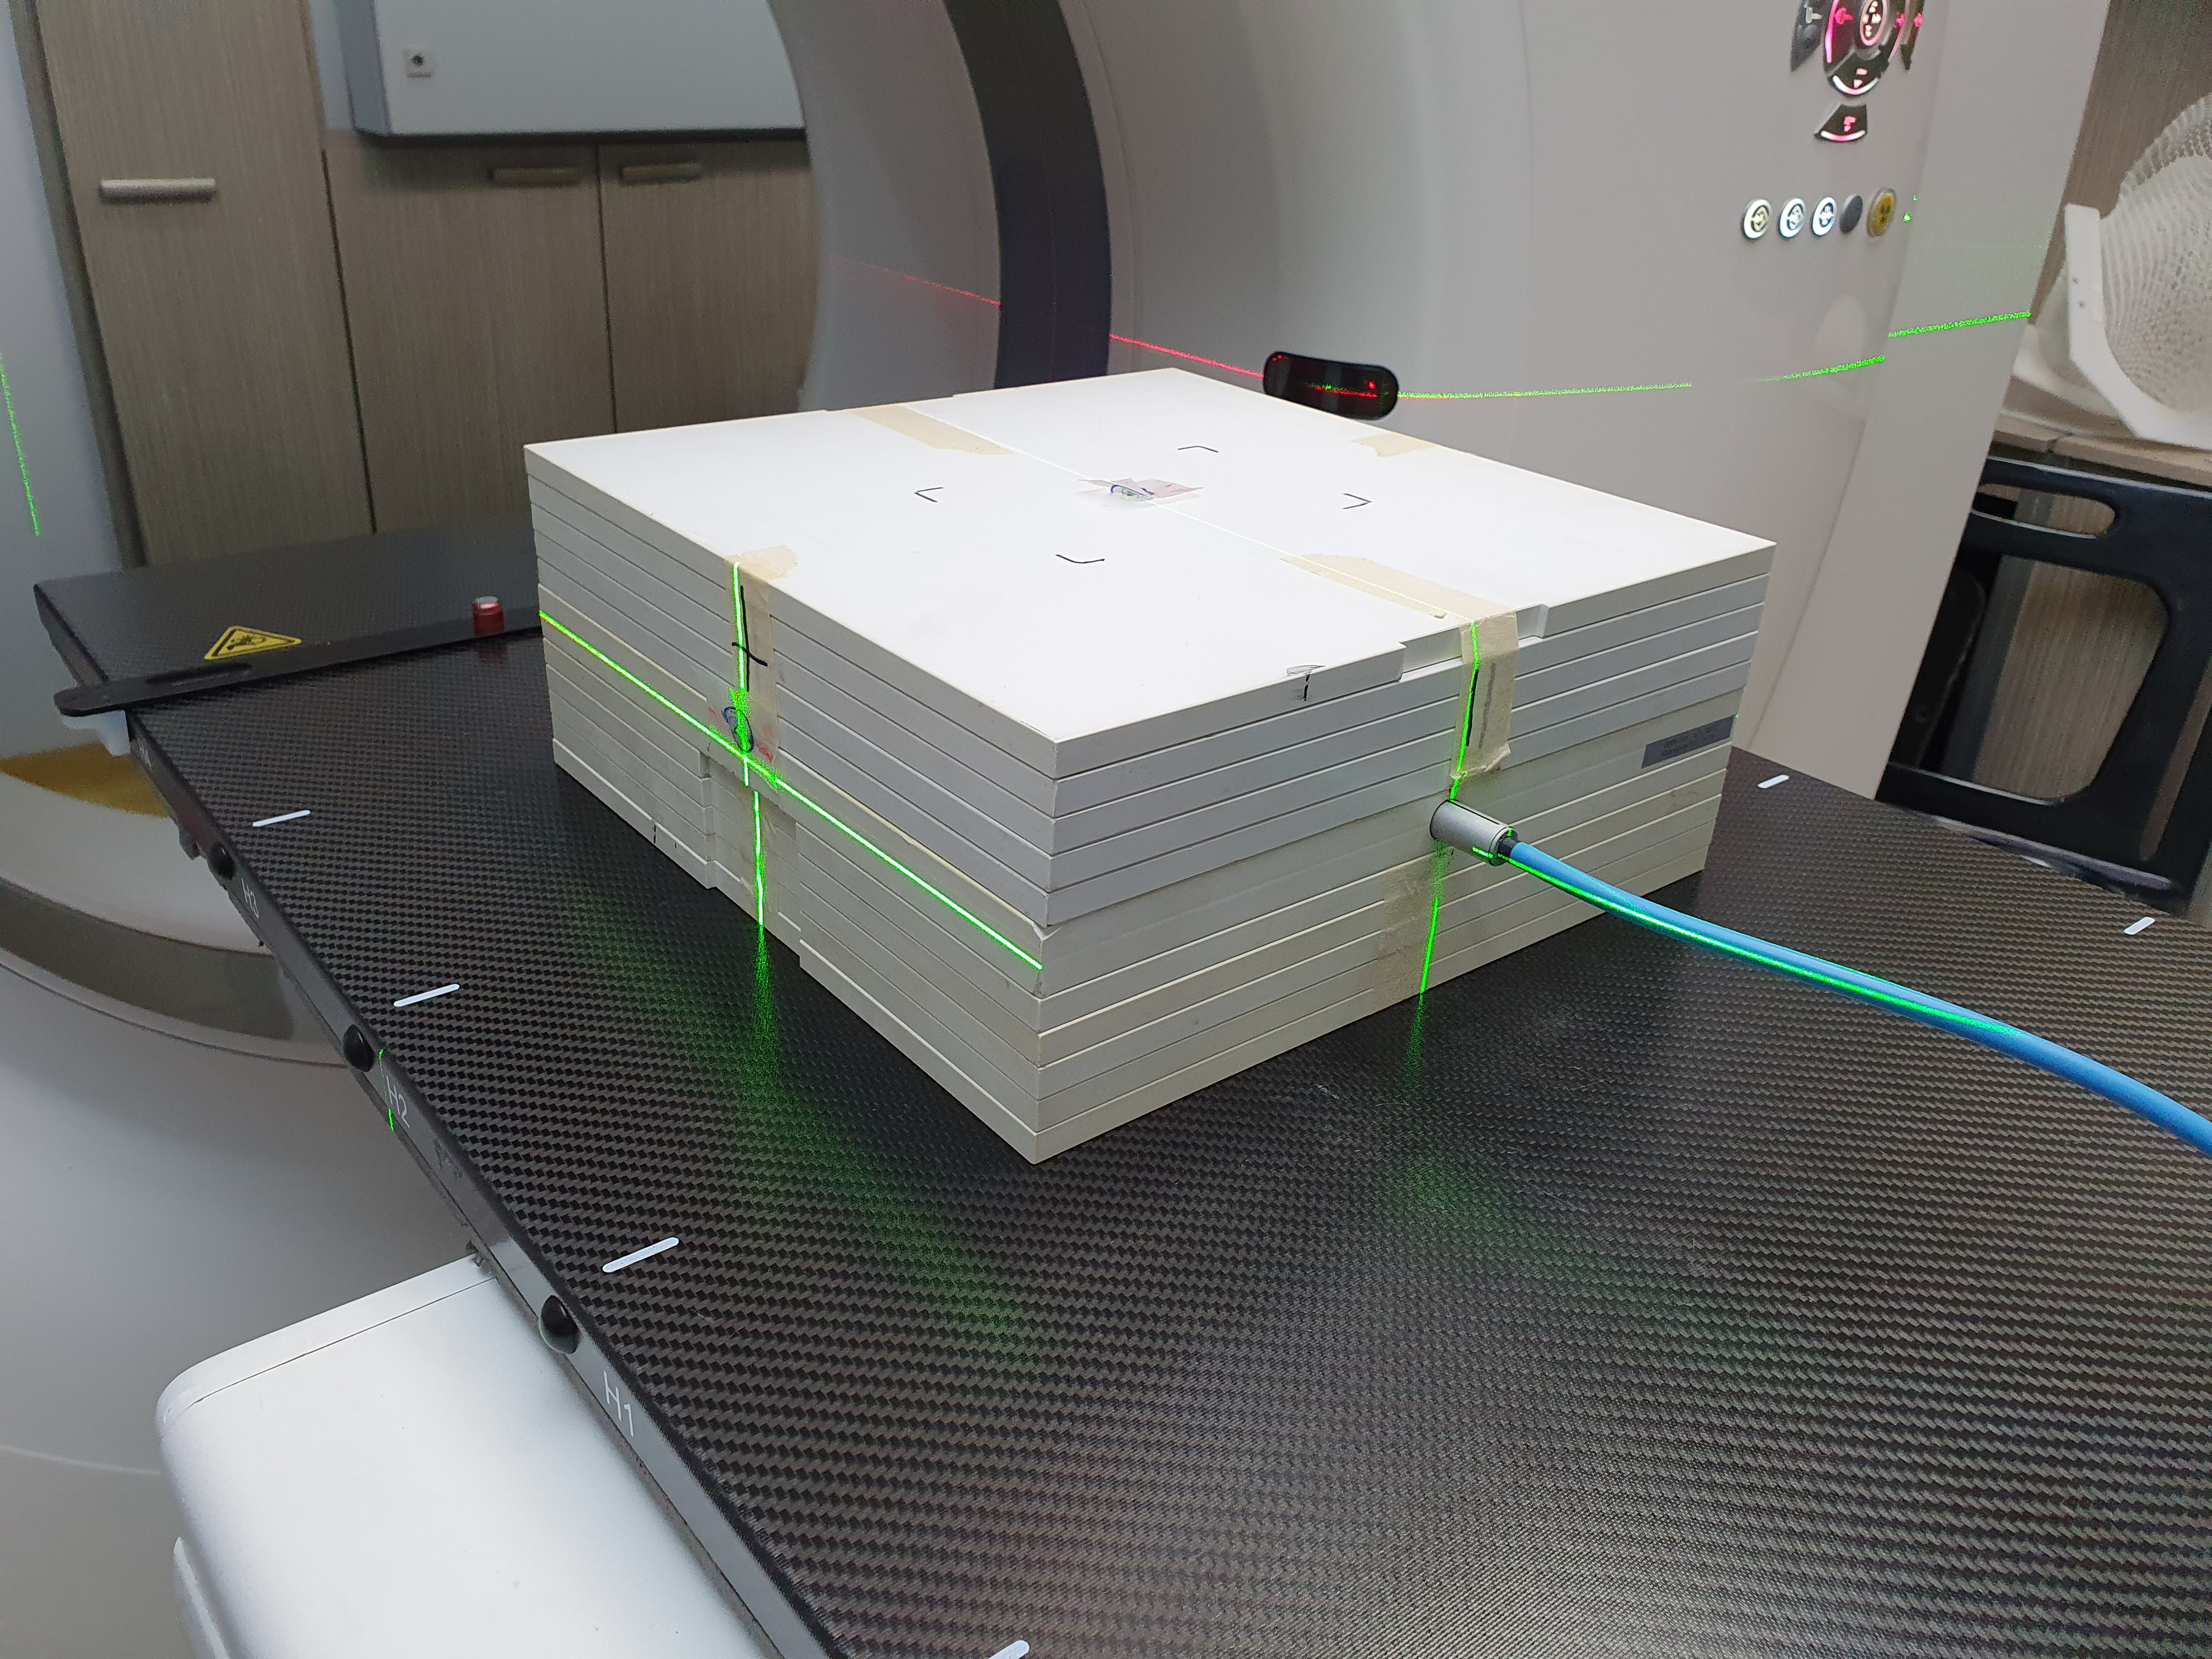
\includegraphics[width=\linewidth]{images/20200826_153715.jpg}
\end{figure}
\end{frame}

\begin{frame}
\begin{figure}
	\centering
	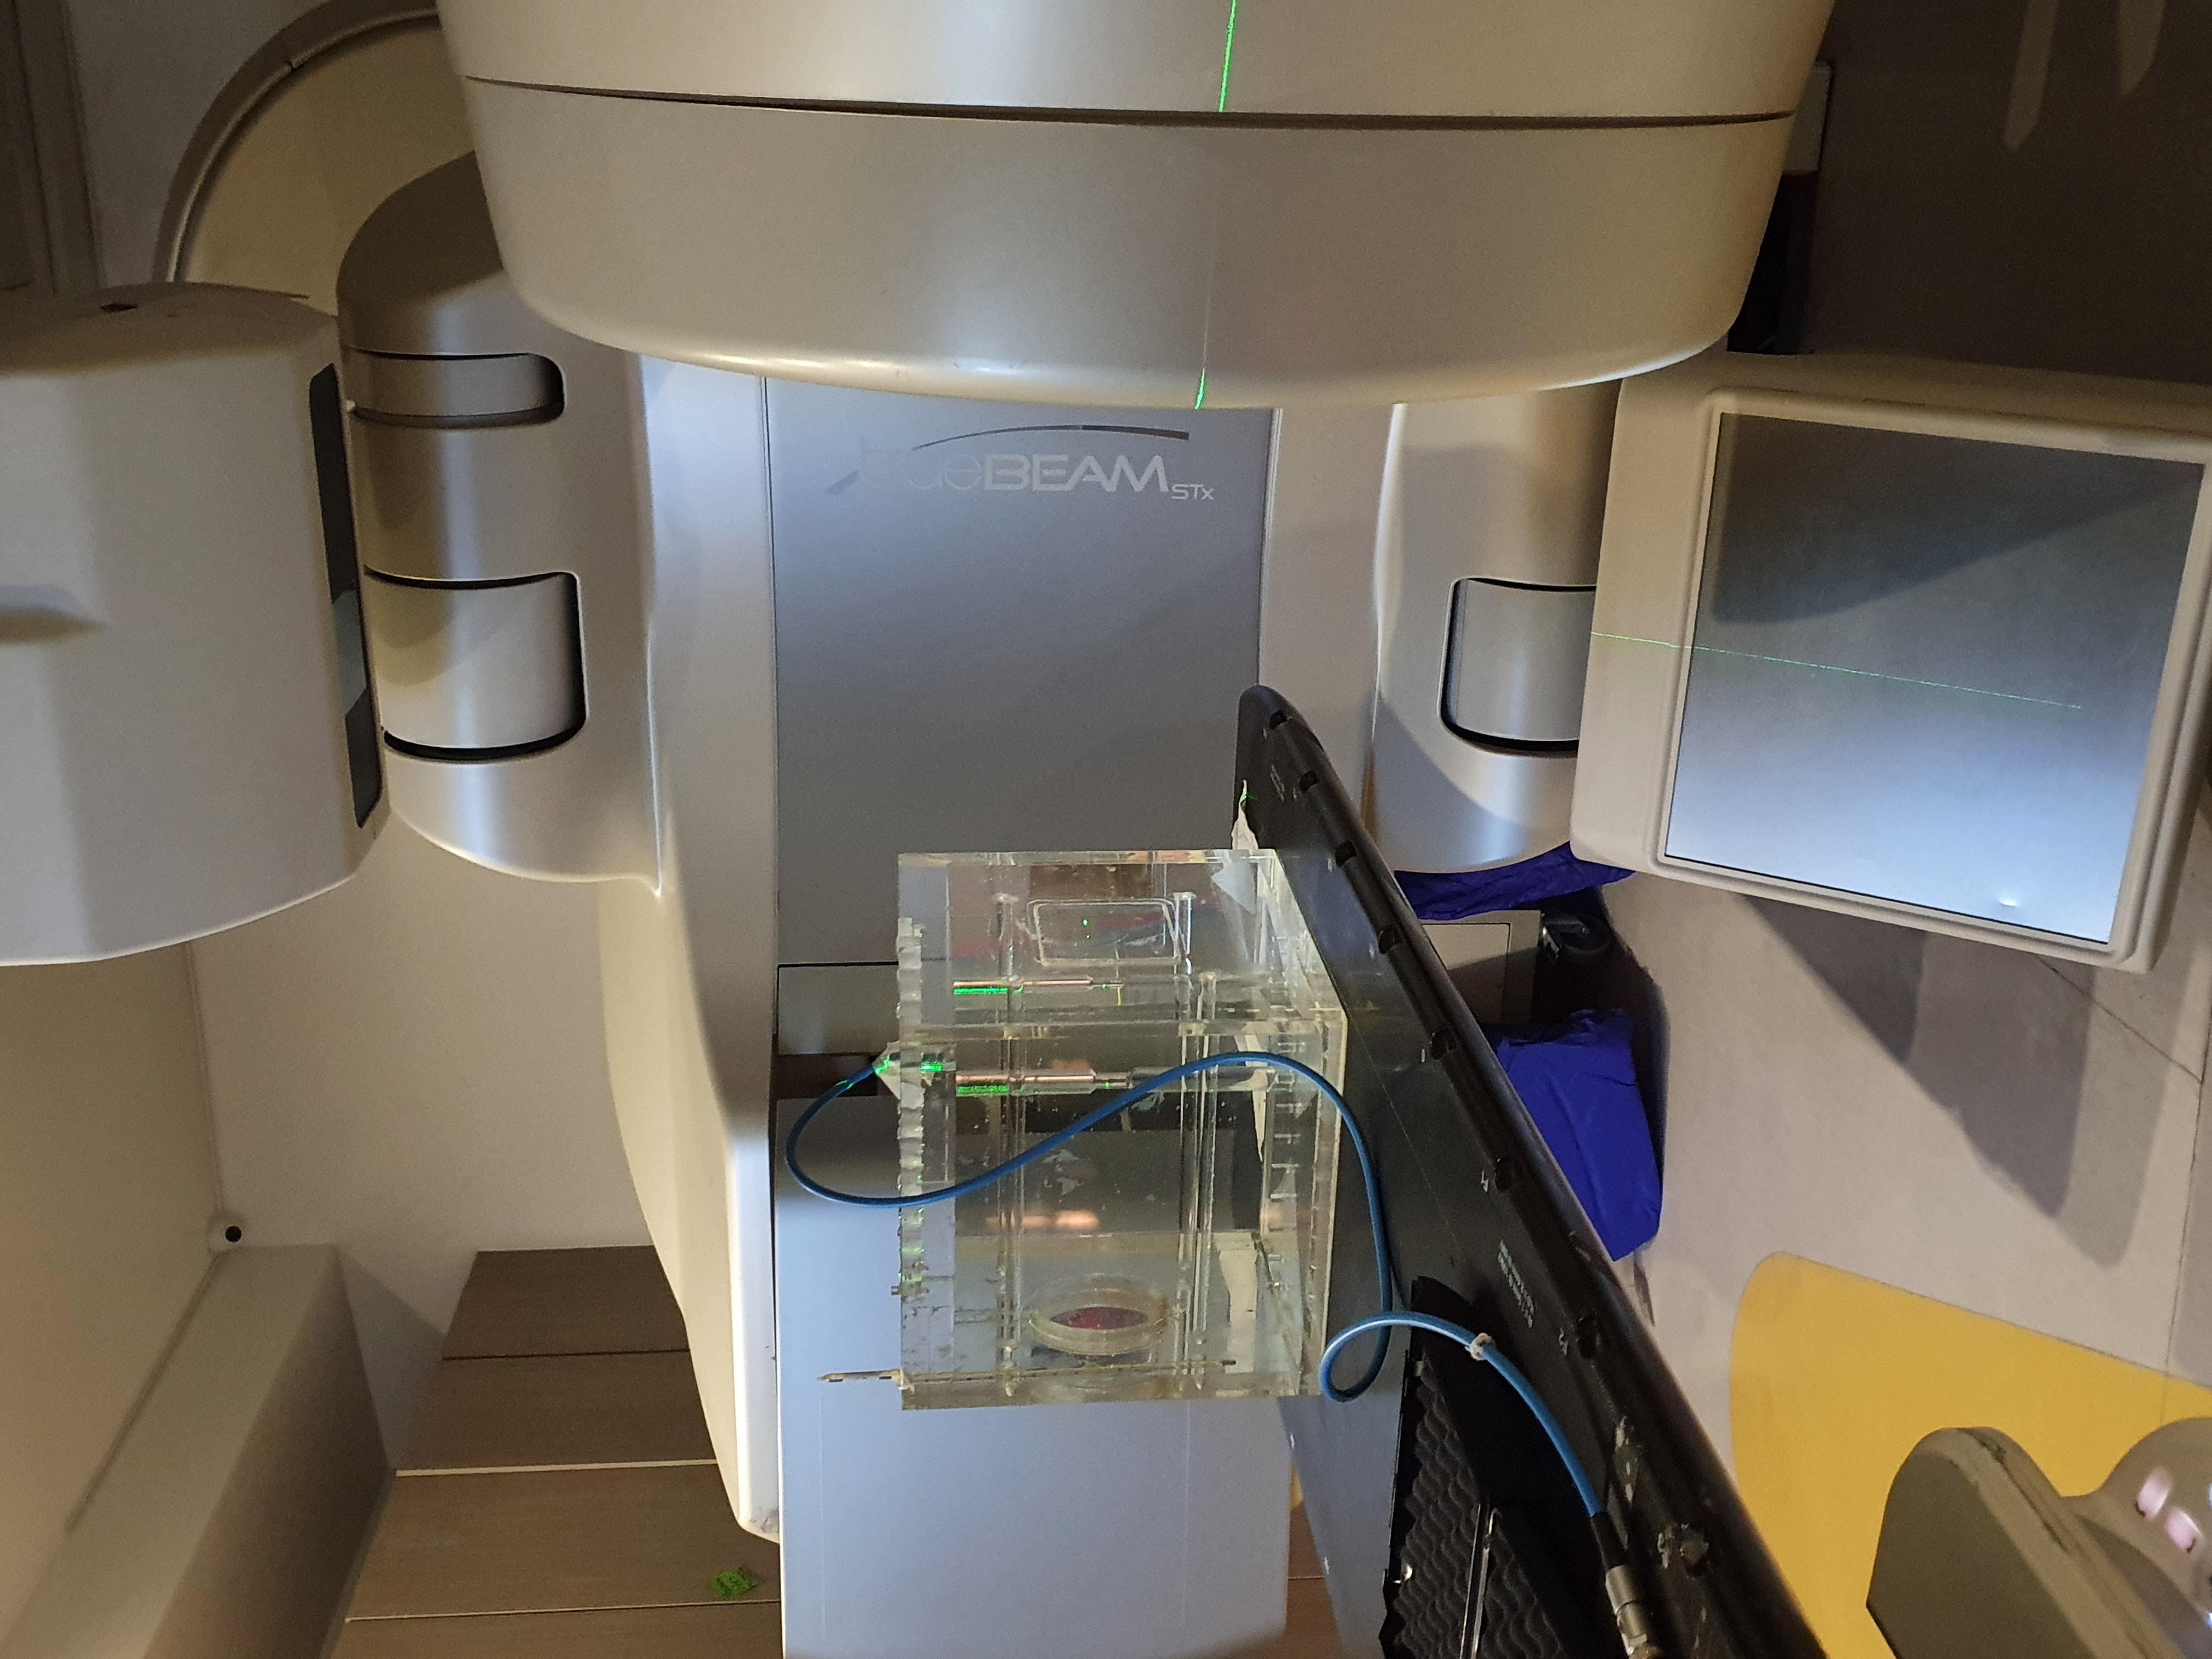
\includegraphics[width=\linewidth]{images/20200826_205548.jpg}
\end{figure}
\end{frame}

\begin{frame}
\begin{figure}
	\centering
	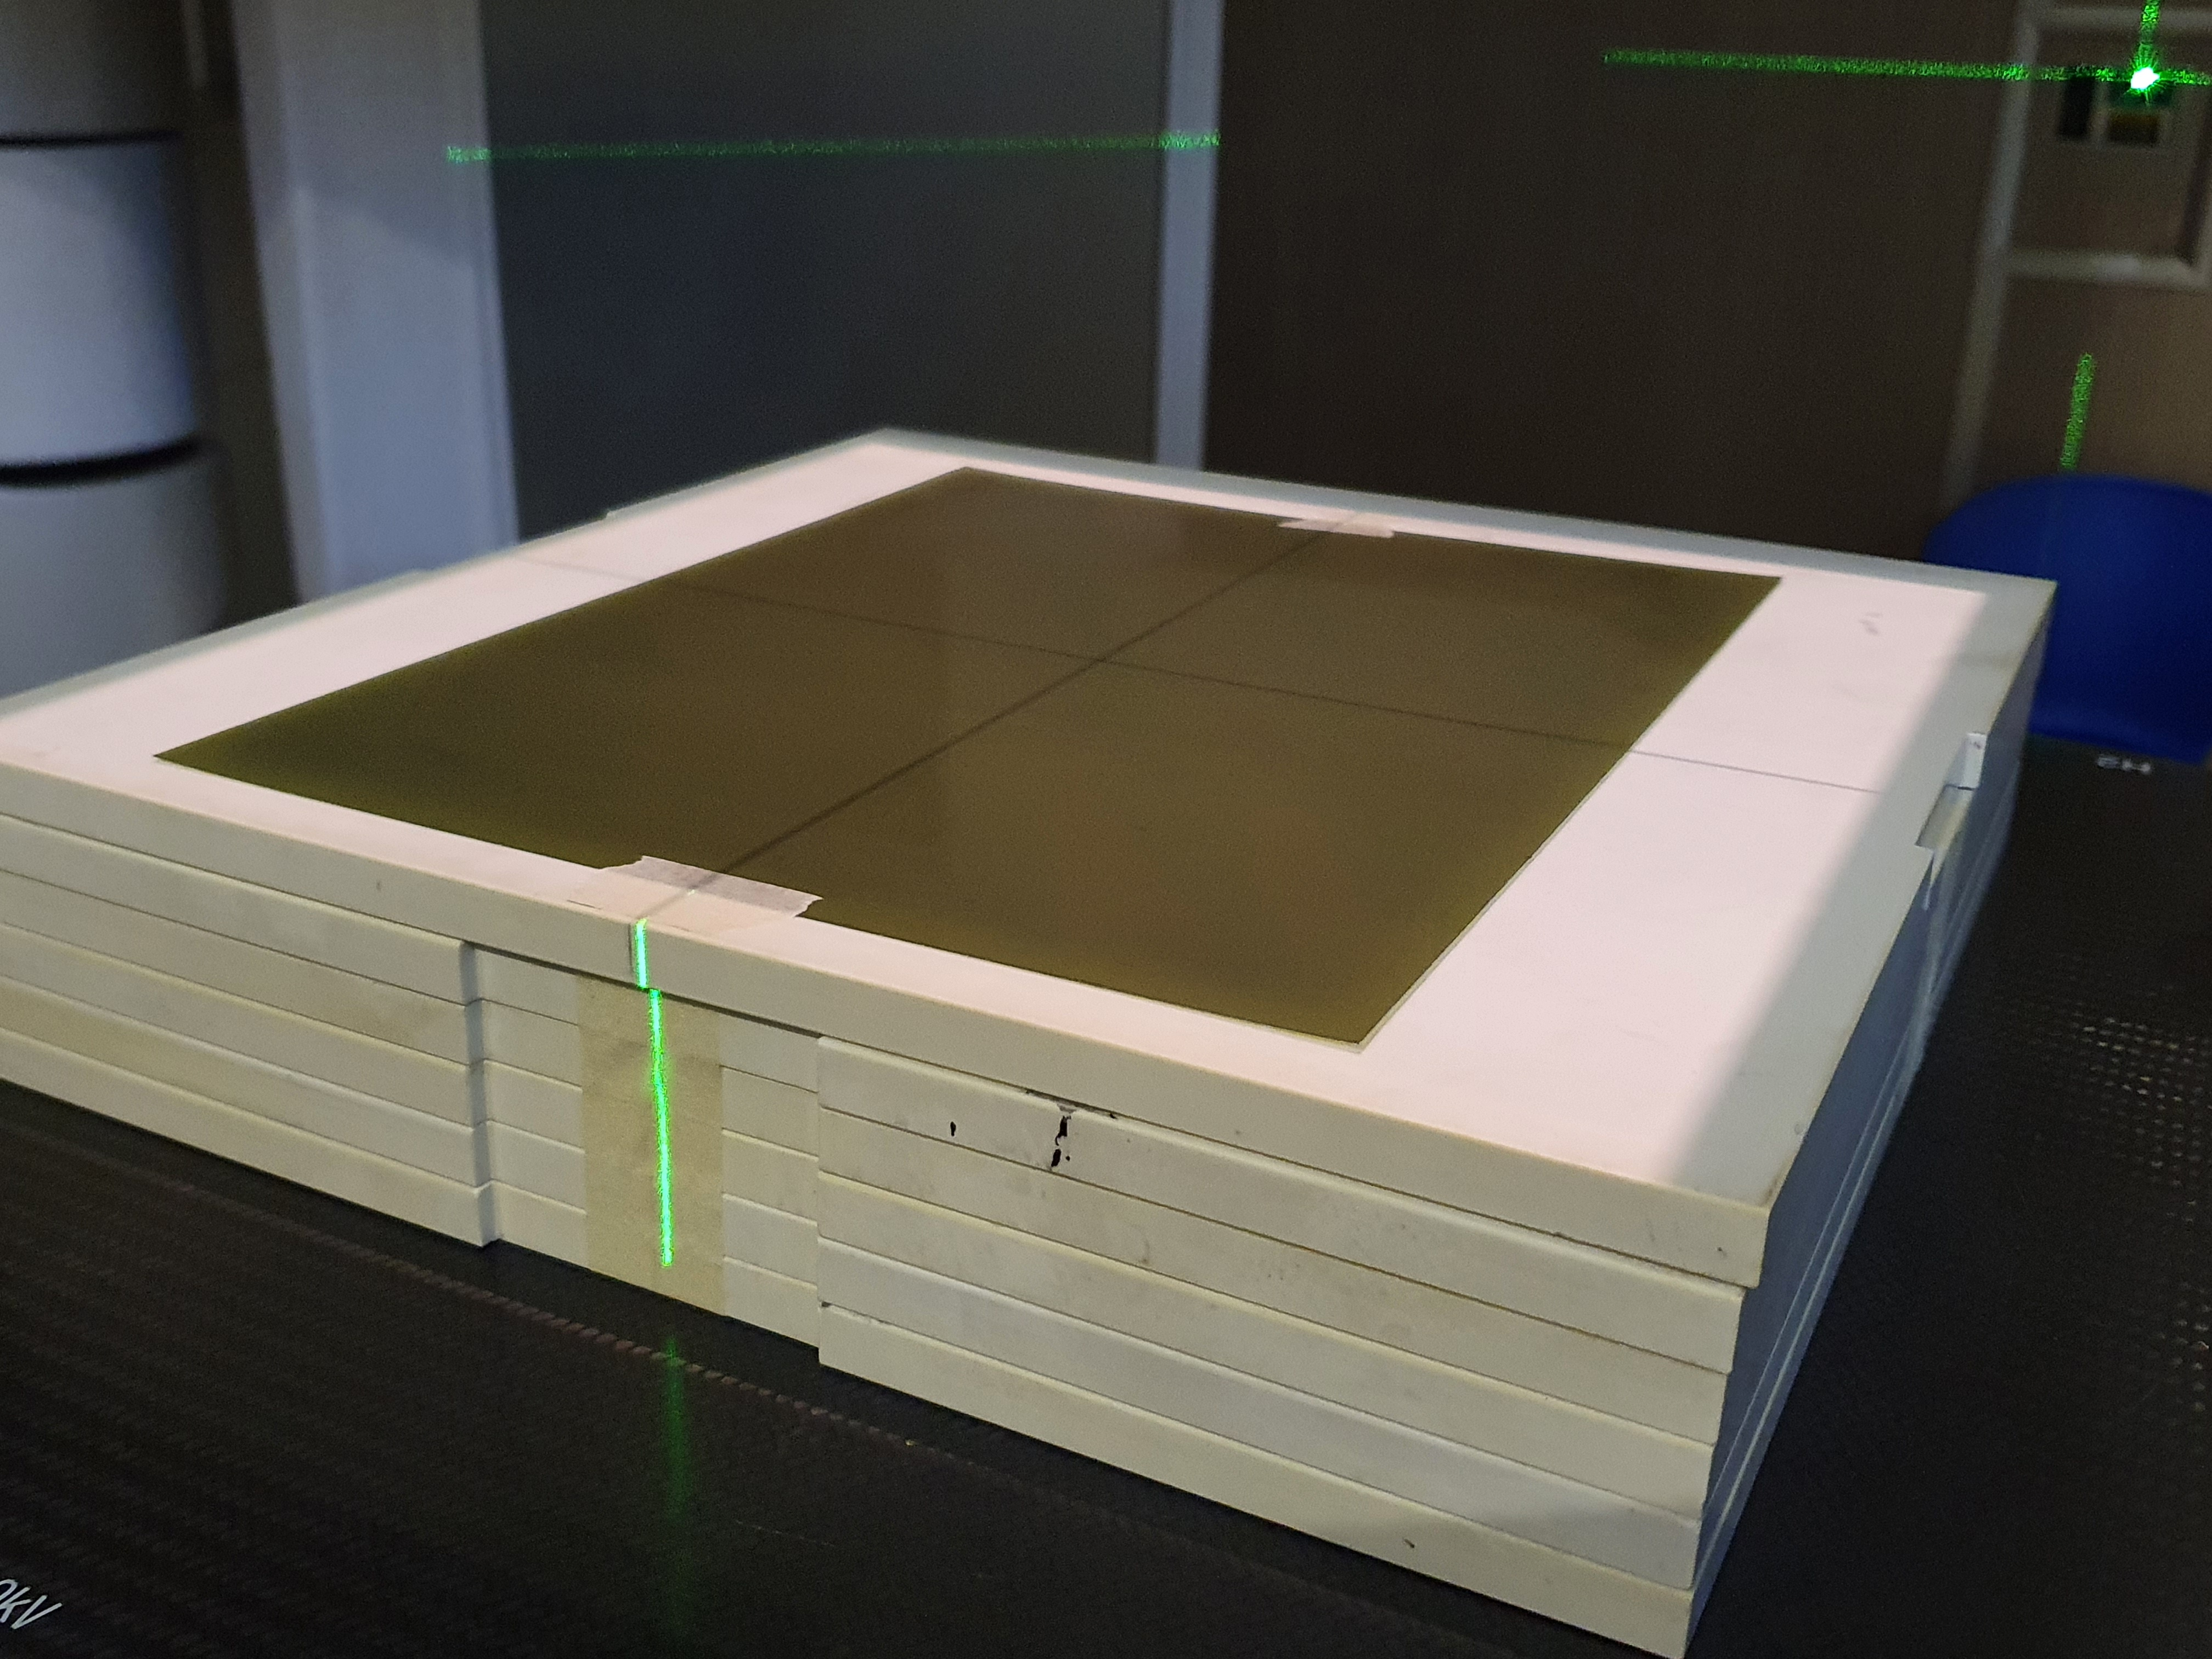
\includegraphics[width=\linewidth]{images/20200826_215214.jpg}
\end{figure}
\end{frame}

\subsection{Desarrollo del software}

\begin{frame}{Programación}
	\begin{figure}
		\centering
		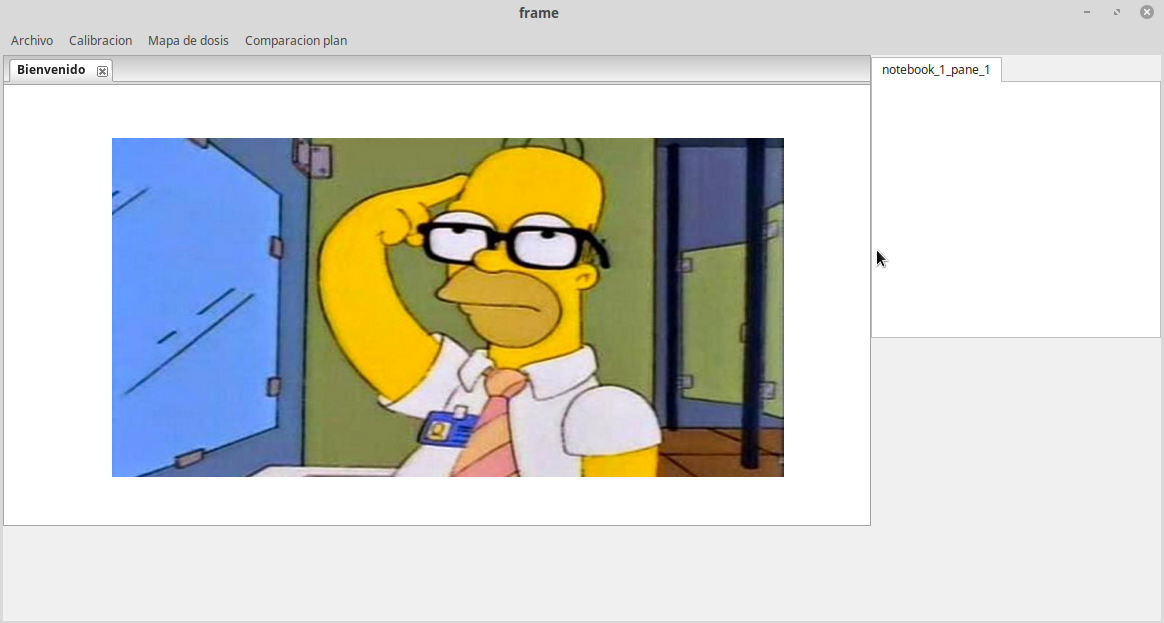
\includegraphics[width=\linewidth]{images/programa1.png}
	\end{figure}
\end{frame}

\begin{frame}
\begin{figure}
	\centering
	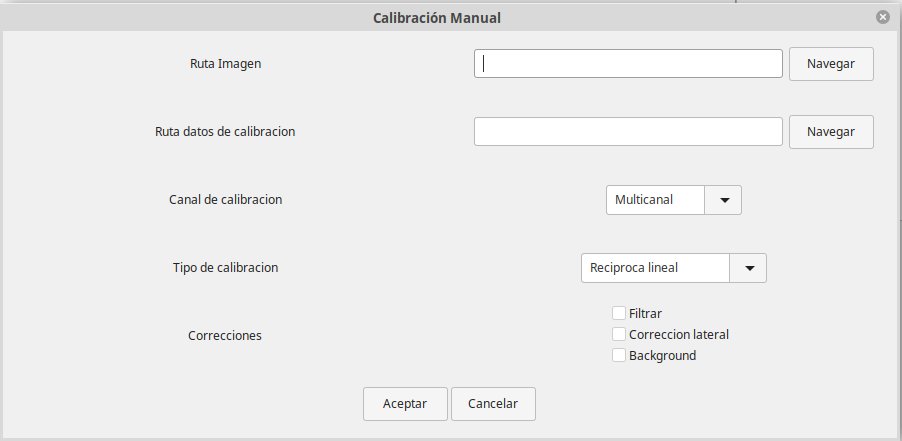
\includegraphics[width=\linewidth]{images/programa2.png}
\end{figure}
\end{frame}

\begin{frame}
\begin{figure}
	\centering
	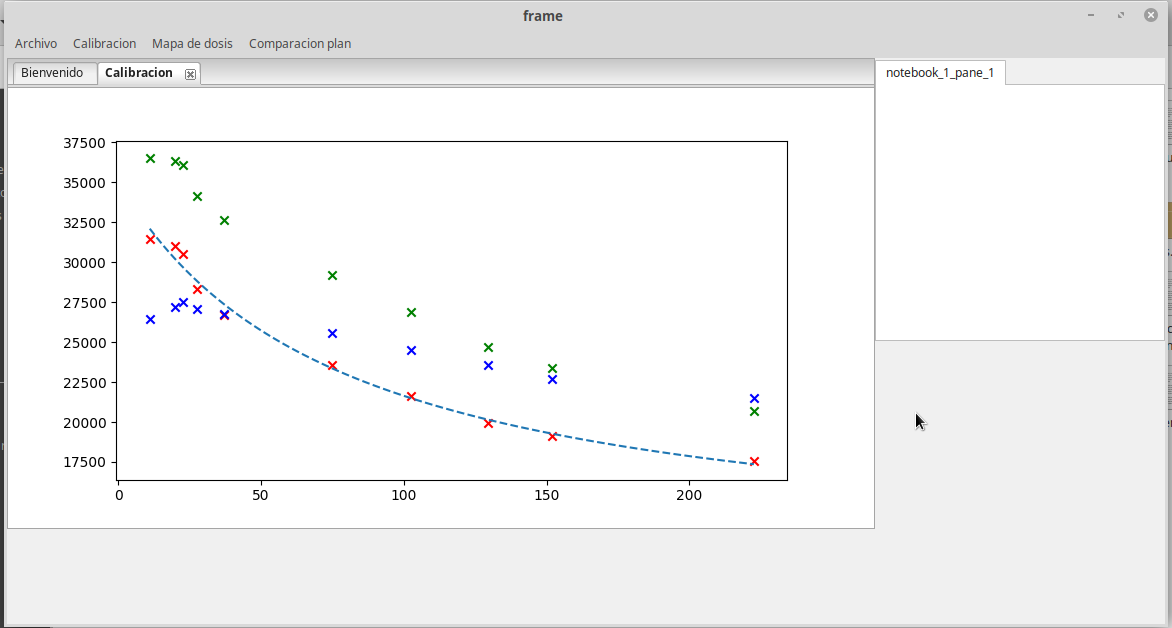
\includegraphics[width=\linewidth]{images/programa3.png}
\end{figure}
\end{frame}


\section{Objetivos a cumplir}
\begin{frame}
\vfill
\centering
\begin{beamercolorbox}[sep=8pt,center,shadow=true,rounded=true]{title}
	\usebeamerfont{title}\insertsectionhead\par%
\end{beamercolorbox}
\vfill
\end{frame}

\begin{frame}
Faltaría lo siguiente
\begin{itemize}
	\item Mejorar la usabilidad del programa
	\item Generar curvas de isodosis
	\item Entender e implementar el cálculo de $\gamma$ para la comparación cuantitativa con los planes de tratamiento
\end{itemize}
\end{frame}



\section{Bibliografia}
\begin{frame}[allowframebreaks]
\frametitle{Referencias}
\nocite{*}
\bibliographystyle{amsalpha}
\bibliography{references}
\end{frame}



\end{document}